% This LaTeX was auto-generated from MATLAB code.
% To make changes, update the MATLAB code and export to LaTeX again.

\documentclass{article}

\usepackage[utf8]{inputenc}
\usepackage[T1]{fontenc}
\usepackage{lmodern}
\usepackage{graphicx}
\usepackage{color}
\usepackage{hyperref}
\usepackage{amsmath}
\usepackage{amsfonts}
\usepackage{epstopdf}
\usepackage[table]{xcolor}
\usepackage{matlab}

\sloppy
\epstopdfsetup{outdir=./}
\graphicspath{ {./testing_images/} }

\begin{document}

\begin{matlabcode}
clear;
clc;
close all;

%% Basic model settings

model.nelx = 40;       % Number of elements in X direction
model.nely = 20;       % Number of elements in Y direction
model.nelz = 6;        % Number of elements in Z direction

% Material properties
model.E0 = 2e9;        % Young's modulus [Pa]
model.Emin = 1e-6*model.E0;
model.nu = 0.30;       % Poisson's ratio

% Create the design domain
design = helper("createDesign",model);

% Display the initial design
helper("showDesign",design);
\end{matlabcode}
\begin{center}
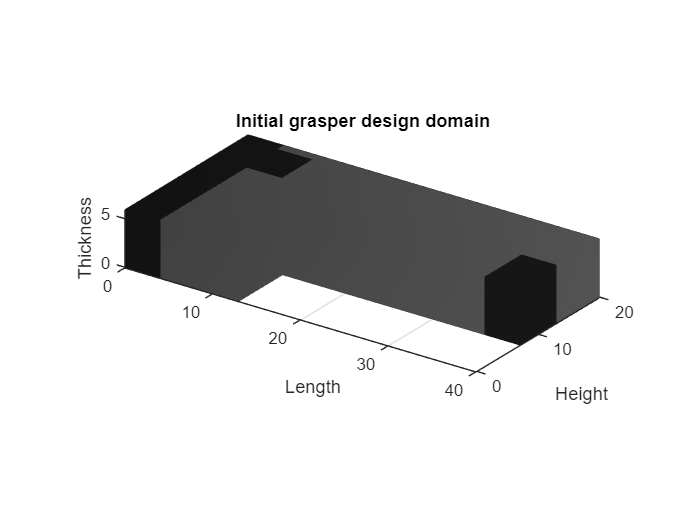
\includegraphics[width=\maxwidth{56.196688409433015em}]{figure_0.png}
\end{center}


\begin{par}
\begin{flushleft}
should get a 3D visualization showing your:
\end{flushleft}
\end{par}

\begin{itemize}
\setlength{\itemsep}{-1ex}
   \item{\begin{flushleft} fixed region,  \end{flushleft}}
   \item{\begin{flushleft} input point,  \end{flushleft}}
   \item{\begin{flushleft} output point. \end{flushleft}}
\end{itemize}

\begin{matlabcode}
%% Boundary conditions

BC = helper("createBC",model,design);

% Display the boundary conditions
helper("showBC",model,design,BC);
\end{matlabcode}
\begin{center}
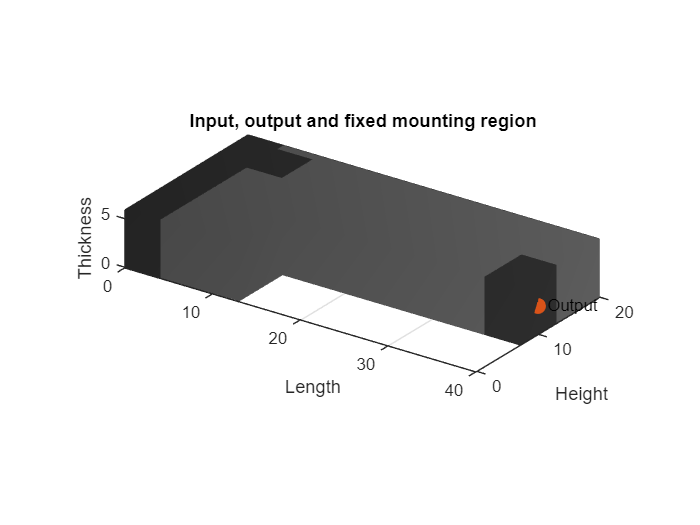
\includegraphics[width=\maxwidth{56.196688409433015em}]{figure_1.png}
\end{center}


\begin{par}
\begin{flushleft}
4. Create the TOP settings
\end{flushleft}
\end{par}

\begin{matlabcode}
%% Topology optimization settings

s.nelx = model.nelx;
s.nely = model.nely;
s.nelz = model.nelz;

% Material
s.E0 = model.E0;
s.Emin = model.Emin;
s.nu = model.nu;

% SIMP parameters
s.penal = 3.0;

% Volume fraction
s.volfrac = 0.40;

% Density filter radius
s.rmin = 2.0;

% Convergence settings
s.maxIter = 50;
s.tolX = 0.01;

% Design and boundary conditions
s.design = design;
s.BC = BC;
\end{matlabcode}


\begin{par}
\begin{flushleft}
5. Run the topology optimization
\end{flushleft}
\end{par}

\begin{matlabcode}
%% Run topology optimization

s.animation.show = true;
s.animation.store = true;
s.animation.threshold = 0.50;
s.animation.every = 1;

result = top3d(s);
\end{matlabcode}
\begin{matlaboutput}
Iteration   1 | objective -1.00335e-10 | volume 0.393 | change 0.100
Iteration   2 | objective -5.85163e-11 | volume 0.400 | change 0.100
Iteration   3 | objective  1.75162e-10 | volume 0.400 | change 0.100
Iteration   4 | objective -1.48055e-09 | volume 0.400 | change 0.100
Iteration   5 | objective -3.59878e-10 | volume 0.393 | change 0.100
Iteration   6 | objective  1.78252e-10 | volume 0.400 | change 0.100
Iteration   7 | objective  1.49824e-11 | volume 0.386 | change 0.100
Iteration   8 | objective -7.71272e-11 | volume 0.386 | change 0.100
Iteration   9 | objective -1.11104e-10 | volume 0.380 | change 0.100
Iteration  10 | objective -2.11917e-10 | volume 0.375 | change 0.100
Iteration  11 | objective -3.35860e-10 | volume 0.375 | change 0.100
Iteration  12 | objective -4.95597e-10 | volume 0.378 | change 0.100
Iteration  13 | objective -8.09366e-10 | volume 0.368 | change 0.100
Iteration  14 | objective -2.22846e-09 | volume 0.356 | change 0.100
Iteration  15 | objective -6.03785e-09 | volume 0.361 | change 0.100
Iteration  16 | objective -1.48800e-08 | volume 0.347 | change 0.100
Iteration  17 | objective -3.90679e-08 | volume 0.340 | change 0.100
Iteration  18 | objective -9.97448e-08 | volume 0.326 | change 0.100
Iteration  19 | objective -2.26473e-07 | volume 0.316 | change 0.100
Iteration  20 | objective -5.96478e-07 | volume 0.314 | change 0.100
Iteration  21 | objective -2.23557e-06 | volume 0.305 | change 0.100
Iteration  22 | objective -3.13986e-06 | volume 0.307 | change 0.100
Iteration  23 | objective -4.42136e-06 | volume 0.311 | change 0.100
Iteration  24 | objective -4.75823e-06 | volume 0.302 | change 0.100
Iteration  25 | objective -5.84424e-06 | volume 0.296 | change 0.100
Iteration  26 | objective -5.96977e-06 | volume 0.287 | change 0.100
Iteration  27 | objective -7.02230e-06 | volume 0.297 | change 0.100
Iteration  28 | objective -7.73848e-06 | volume 0.287 | change 0.100
Iteration  29 | objective -8.72764e-06 | volume 0.293 | change 0.100
Iteration  30 | objective -9.18985e-06 | volume 0.285 | change 0.100
Iteration  31 | objective -1.04400e-05 | volume 0.280 | change 0.100
Iteration  32 | objective -1.12331e-05 | volume 0.273 | change 0.100
Iteration  33 | objective -1.18799e-05 | volume 0.274 | change 0.100
Iteration  34 | objective -1.20756e-05 | volume 0.268 | change 0.100
Iteration  35 | objective -1.20488e-05 | volume 0.262 | change 0.100
Iteration  36 | objective -1.30669e-05 | volume 0.258 | change 0.100
Iteration  37 | objective -1.46986e-05 | volume 0.253 | change 0.100
Iteration  38 | objective -1.34856e-05 | volume 0.248 | change 0.100
Iteration  39 | objective -1.50215e-05 | volume 0.240 | change 0.100
Iteration  40 | objective -1.37308e-05 | volume 0.234 | change 0.100
Iteration  41 | objective -1.39706e-05 | volume 0.228 | change 0.100
Iteration  42 | objective -2.02984e-05 | volume 0.223 | change 0.100
Iteration  43 | objective -1.48827e-05 | volume 0.218 | change 0.100
Iteration  44 | objective -1.70120e-05 | volume 0.216 | change 0.100
Iteration  45 | objective -1.60493e-05 | volume 0.212 | change 0.100
Iteration  46 | objective -3.58388e-05 | volume 0.207 | change 0.100
Iteration  47 | objective -1.60462e-05 | volume 0.203 | change 0.100
Iteration  48 | objective -1.68524e-05 | volume 0.201 | change 0.100
Iteration  49 | objective -2.65448e-05 | volume 0.197 | change 0.100
Iteration  50 | objective -1.81929e-05 | volume 0.195 | change 0.100
\end{matlaboutput}
\begin{center}
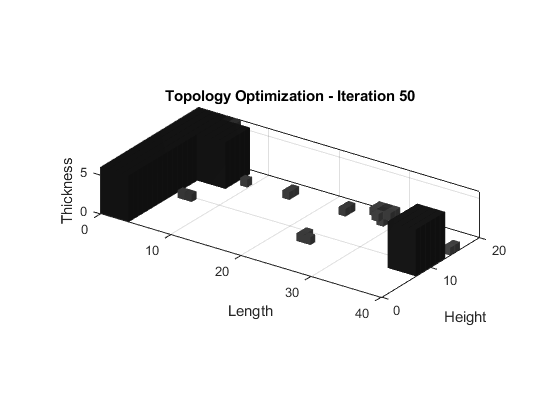
\includegraphics[width=\maxwidth{56.196688409433015em}]{figure_2.png}
\end{center}


\begin{par}
\begin{flushleft}
6. Display the final topology
\end{flushleft}
\end{par}

\begin{matlabcode}
%% Display final topology

threshold = 0.50;

helper("showTopology",result.xPhys,threshold);
\end{matlabcode}
\begin{center}
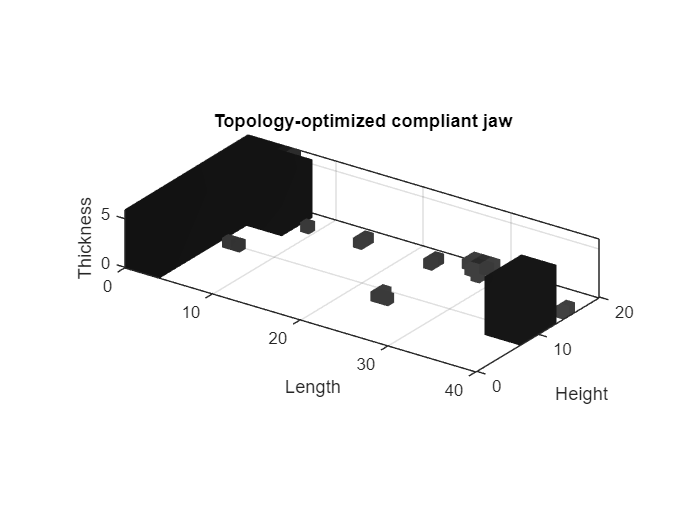
\includegraphics[width=\maxwidth{56.196688409433015em}]{figure_3.png}
\end{center}


\begin{par}
\begin{flushleft}
7. Plot the optimization history
\end{flushleft}
\end{par}

\begin{matlabcode}
%% Plot convergence history

helper("plotHistory",result);
\end{matlabcode}
\begin{center}
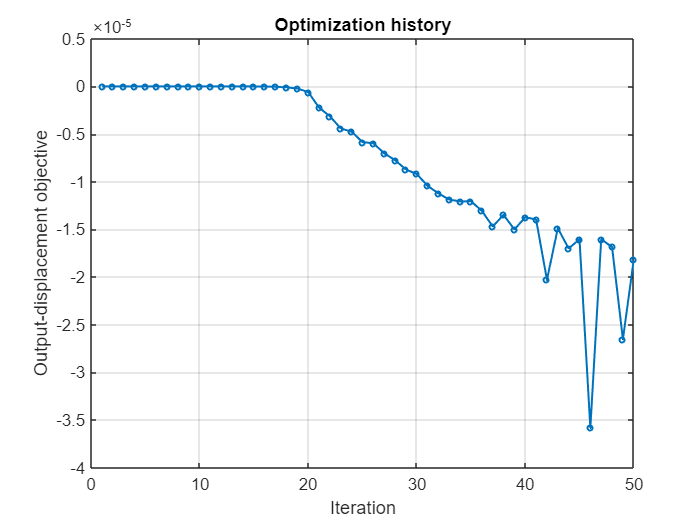
\includegraphics[width=\maxwidth{56.196688409433015em}]{figure_4.png}
\end{center}
\begin{center}
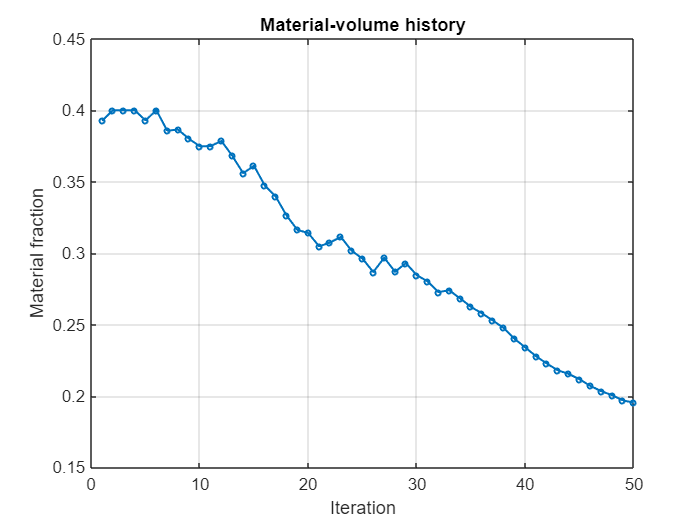
\includegraphics[width=\maxwidth{56.196688409433015em}]{figure_5.png}
\end{center}


\begin{par}
\begin{flushleft}
8. Check the basic displacement response
\end{flushleft}
\end{par}

\begin{matlabcode}
%% Basic displacement response

displacement = linspace(0,1,20);

response = helper("forceResponse",result,displacement);
\end{matlabcode}
\begin{matlaboutput}
Normalized input stiffness: 14264.131471
Output/input displacement ratio: -0.286239
\end{matlaboutput}
\begin{matlabcode}

helper("plotForceResponse",response);
\end{matlabcode}
\begin{center}
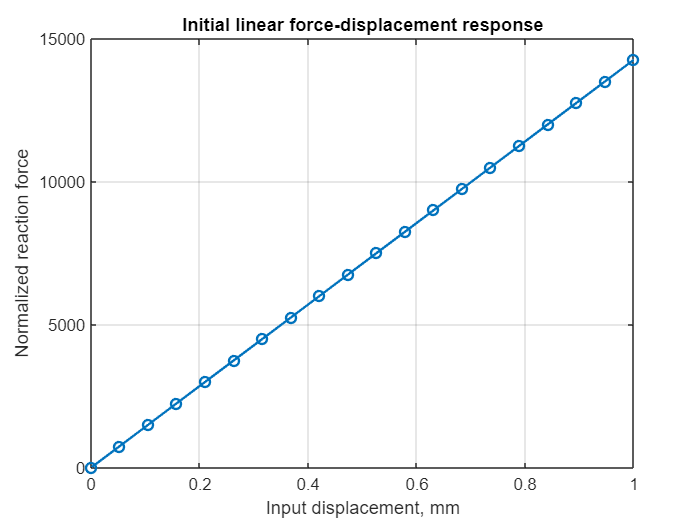
\includegraphics[width=\maxwidth{56.196688409433015em}]{figure_6.png}
\end{center}


\begin{par}
\begin{flushleft}
9. Export the optimized topology as STL
\end{flushleft}
\end{par}

\begin{matlabcode}
%% Export STL

elementSize = 1.0;   % Element size in your chosen geometry units
fileName = "optimized_grasper.stl";

helper("exportSTL", ...
       result.xPhys, ...
       threshold, ...
       elementSize, ...
       fileName);
\end{matlabcode}

\end{document}
